\documentclass[10pt,a4paper,twocolumn,twoside]{tau-class/tau}

% --- PACKAGES ---
\usepackage[english]{babel}
\usepackage{graphicx}         % For images
\usepackage{booktabs}         % For professional tables
\usepackage{fontawesome5}     % For icons (e.g., GitHub, LinkedIn)
\usepackage{enumitem}         % For list customization
\usepackage{titlesec}         % For section title spacing
\usepackage{caption}          % For caption customization
\usepackage{hyperref}         % For clickable links (should be loaded last)

% --- DOCUMENT SETTINGS ---
% Set the path for images to keep the code clean
\graphicspath{{figures/}}

% Reduce spacing around floats and section titles for a compact report
\setlength{\textfloatsep}{8pt plus 1.0pt minus 2.0pt}
\setlength{\floatsep}{6pt plus 1.0pt minus 2.0pt}
\setlength{\intextsep}{6pt plus 1.0pt minus 2.0pt}
\titlespacing*{\section}{0pt}{*1.2}{*0.8}
\titlespacing*{\subsection}{0pt}{*1.0}{*0.5}
\captionsetup[table]{skip=2pt}

%----------------------------------------------------------
% TITLE 
%----------------------------------------------------------
\journalname{Summary Report}
\title{Credit Card Fraud Detection}

%----------------------------------------------------------
% AUTHORS, AFFILIATIONS AND PROFESSOR
%----------------------------------------------------------
\author[1]{Omar Ayman Tawfiq Bakr \href{mailto:bakro0298@gmail.com}{\faGoogle}\hspace{0.5em}
 \href{https://www.linkedin.com/in/omarrbakr/}{\faLinkedinIn}\hspace{0.5em} \href{https://github.com/omarTBakr}{\faGithub}}

%----------------------------------------------------------
% FOOTER INFORMATION
%----------------------------------------------------------
\footinfo{Summary Report}
\theday{May 21, 2025}
\leadauthor{Omar Ayman Bakr}
\course{Credit Card Fraud Detection Report}

%----------------------------------------------------------
\begin{document}
%----------------------------------------------------------
        
    \maketitle
    \thispagestyle{firststyle}
    
    \begin{abstract}    
        This report summarizes findings from the Kaggle Credit Card Fraud Detection dataset (\href{https://www.kaggle.com/datasets/mlg-ulb/creditcardfraud}{link}). Boosting algorithms proved most effective, with the top model achieving an F1-score of 0.89 on the highly imbalanced test set.
    \end{abstract}

    \keywords{EDA, data analysis, machine learning, AI, data exploration, imbalanced data, boosting algorithms, tree-based algorithms, Logistic Regression, Neural networks, Focal loss}

%----------------------------------------------------------
\section{Introduction}
Credit Card Fraud Detection is a classification problem using a Kaggle dataset with mostly anonymized features. The goal is to identify fraudulent transactions.
\begin{itemize}[noitemsep] % 'noitemsep' makes the list more compact
    \item Features \texttt{V1}--\texttt{V28}: anonymized
    \item \texttt{Time}: Seconds since first transaction
    \item \texttt{Amount}: Transaction amount
    \item \texttt{Class}: 1 = Fraud, 0 = Normal
\end{itemize}

\section{Methods}
A range of models were evaluated to compare their performance on imbalanced data, including variants with focal loss.
\begin{itemize}[noitemsep]
    \item Tree-based: Decision Trees, Random Forest
    \item Boosting: AdaBoost, CatBoost, LightGBM, XGBoost, XGBRF
    \item Logistic Regression (log loss, focal loss)
    \item Neural Network (focal loss)
    \item Voting classifier (ensemble)
\end{itemize}

\section{Data Insights}
\textbf{Feature Distribution:} Most features have similar means; some (e.g., V8, V23) show outliers. Only 92 out of 57,010 transactions are fraud.

\begin{figure}[htbp] % Use [htbp] for better float placement
    \centering
    \includegraphics[width=0.95\linewidth]{violonPlotForData.png}
    \caption{Distribution for all anonymous features.}
    \label{fig:distribution-data}
\end{figure}

\textbf{Imbalance:} The dataset is extremely imbalanced (\textless0.2\% fraud), as shown in Figures~\ref{fig:bar-imbalance} and \ref{fig:pie-imbalance}.

\begin{figure}[htbp]
    \centering
    \includegraphics[width=0.95\linewidth]{barPlot.png}
    \caption{Fraud vs Non-Fraud Cases.}
    \label{fig:bar-imbalance}
\end{figure}

\begin{figure}[htbp]
    \centering
    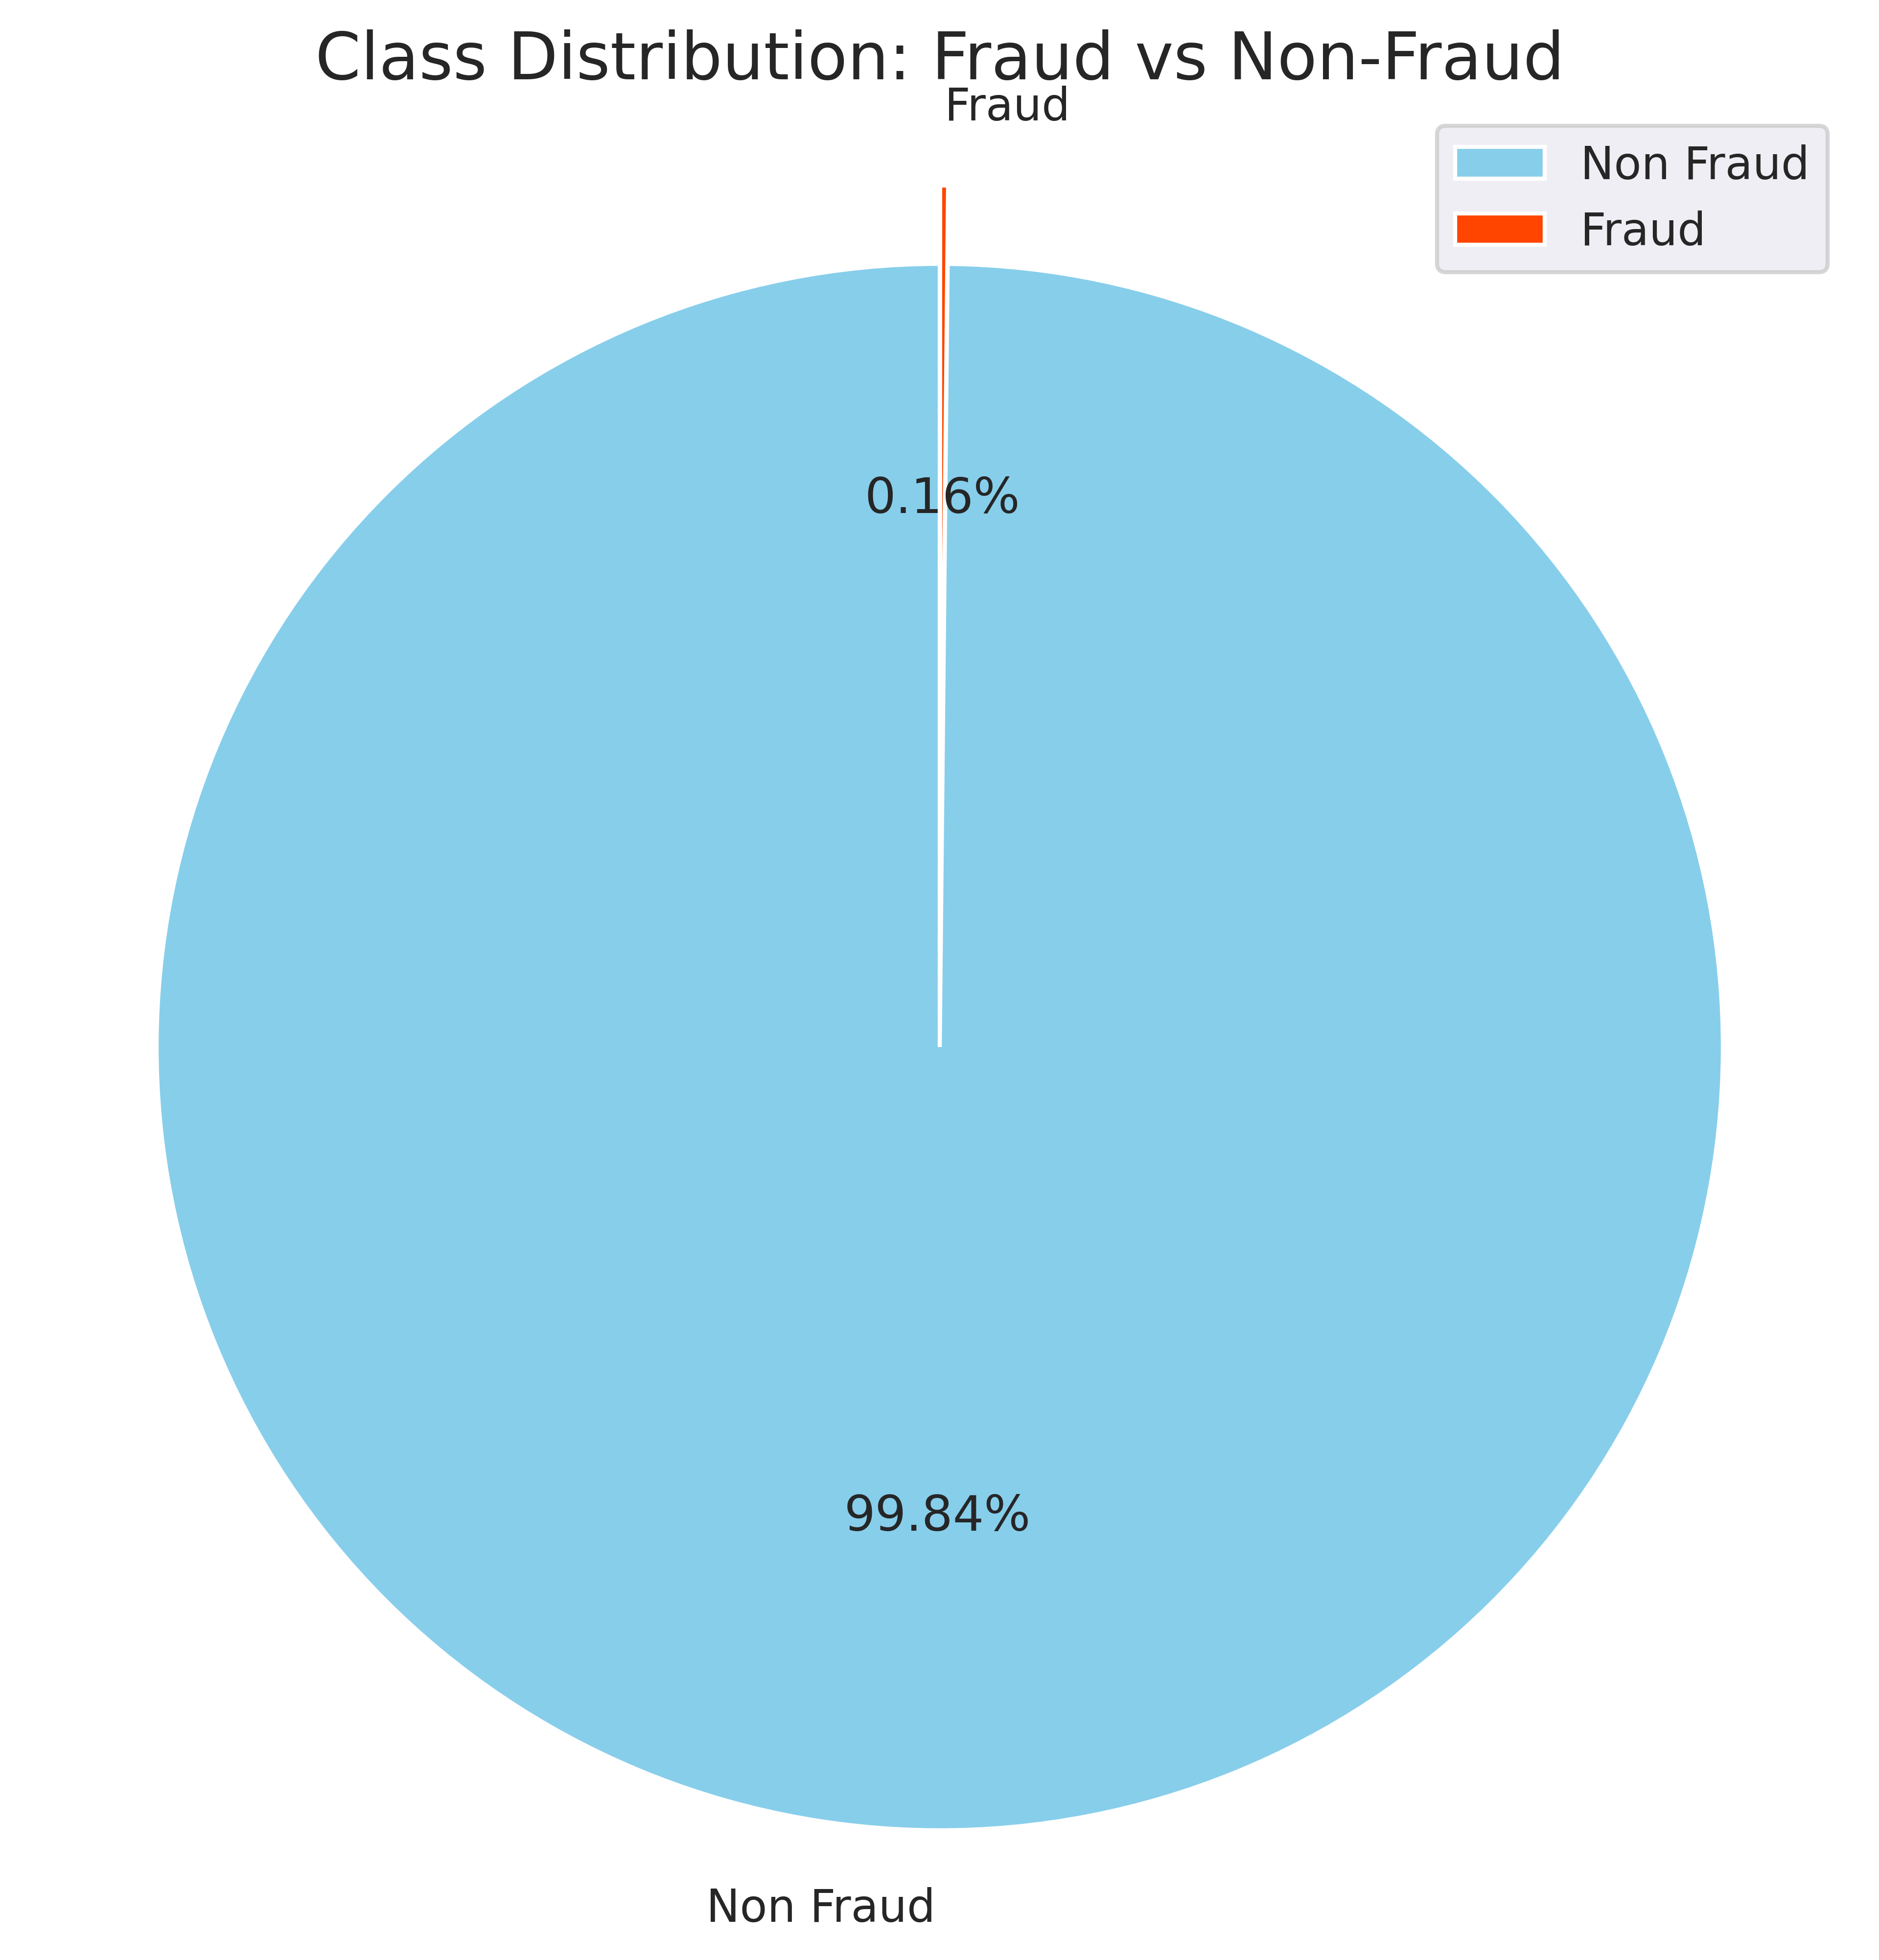
\includegraphics[width=0.95\linewidth]{pieChart.png}
    \caption{Class Distribution: Fraud vs Non-Fraud.}
    \label{fig:pie-imbalance}
\end{figure}

\textbf{2D Projection:} A t-SNE projection (Figure~\ref{fig:tsne-imbalance}) shows no clear separation for fraud cases, indicating a complex, non-linear boundary.

\begin{figure}[htbp]
    \centering
    \includegraphics[width=0.95\linewidth]{tsne2D.png}
    \caption{2D projection using t-SNE.}
    \label{fig:tsne-imbalance}
\end{figure}

\section{Modeling and Results}
% --- SMOOTH INTEGRATION ---
Most boosting algorithms achieved F1 scores above 0.85, significantly outperforming other model families. Notably, XGBoost was the top-performing model with an F1 score of 0.89. Its strong performance across key metrics is visualized in Figure~\ref{fig:xgboost_results}, which displays the detailed Precision-Recall and ROC curves, confirming its ability to effectively distinguish between classes.

\begin{figure}[htbp]
    \centering
    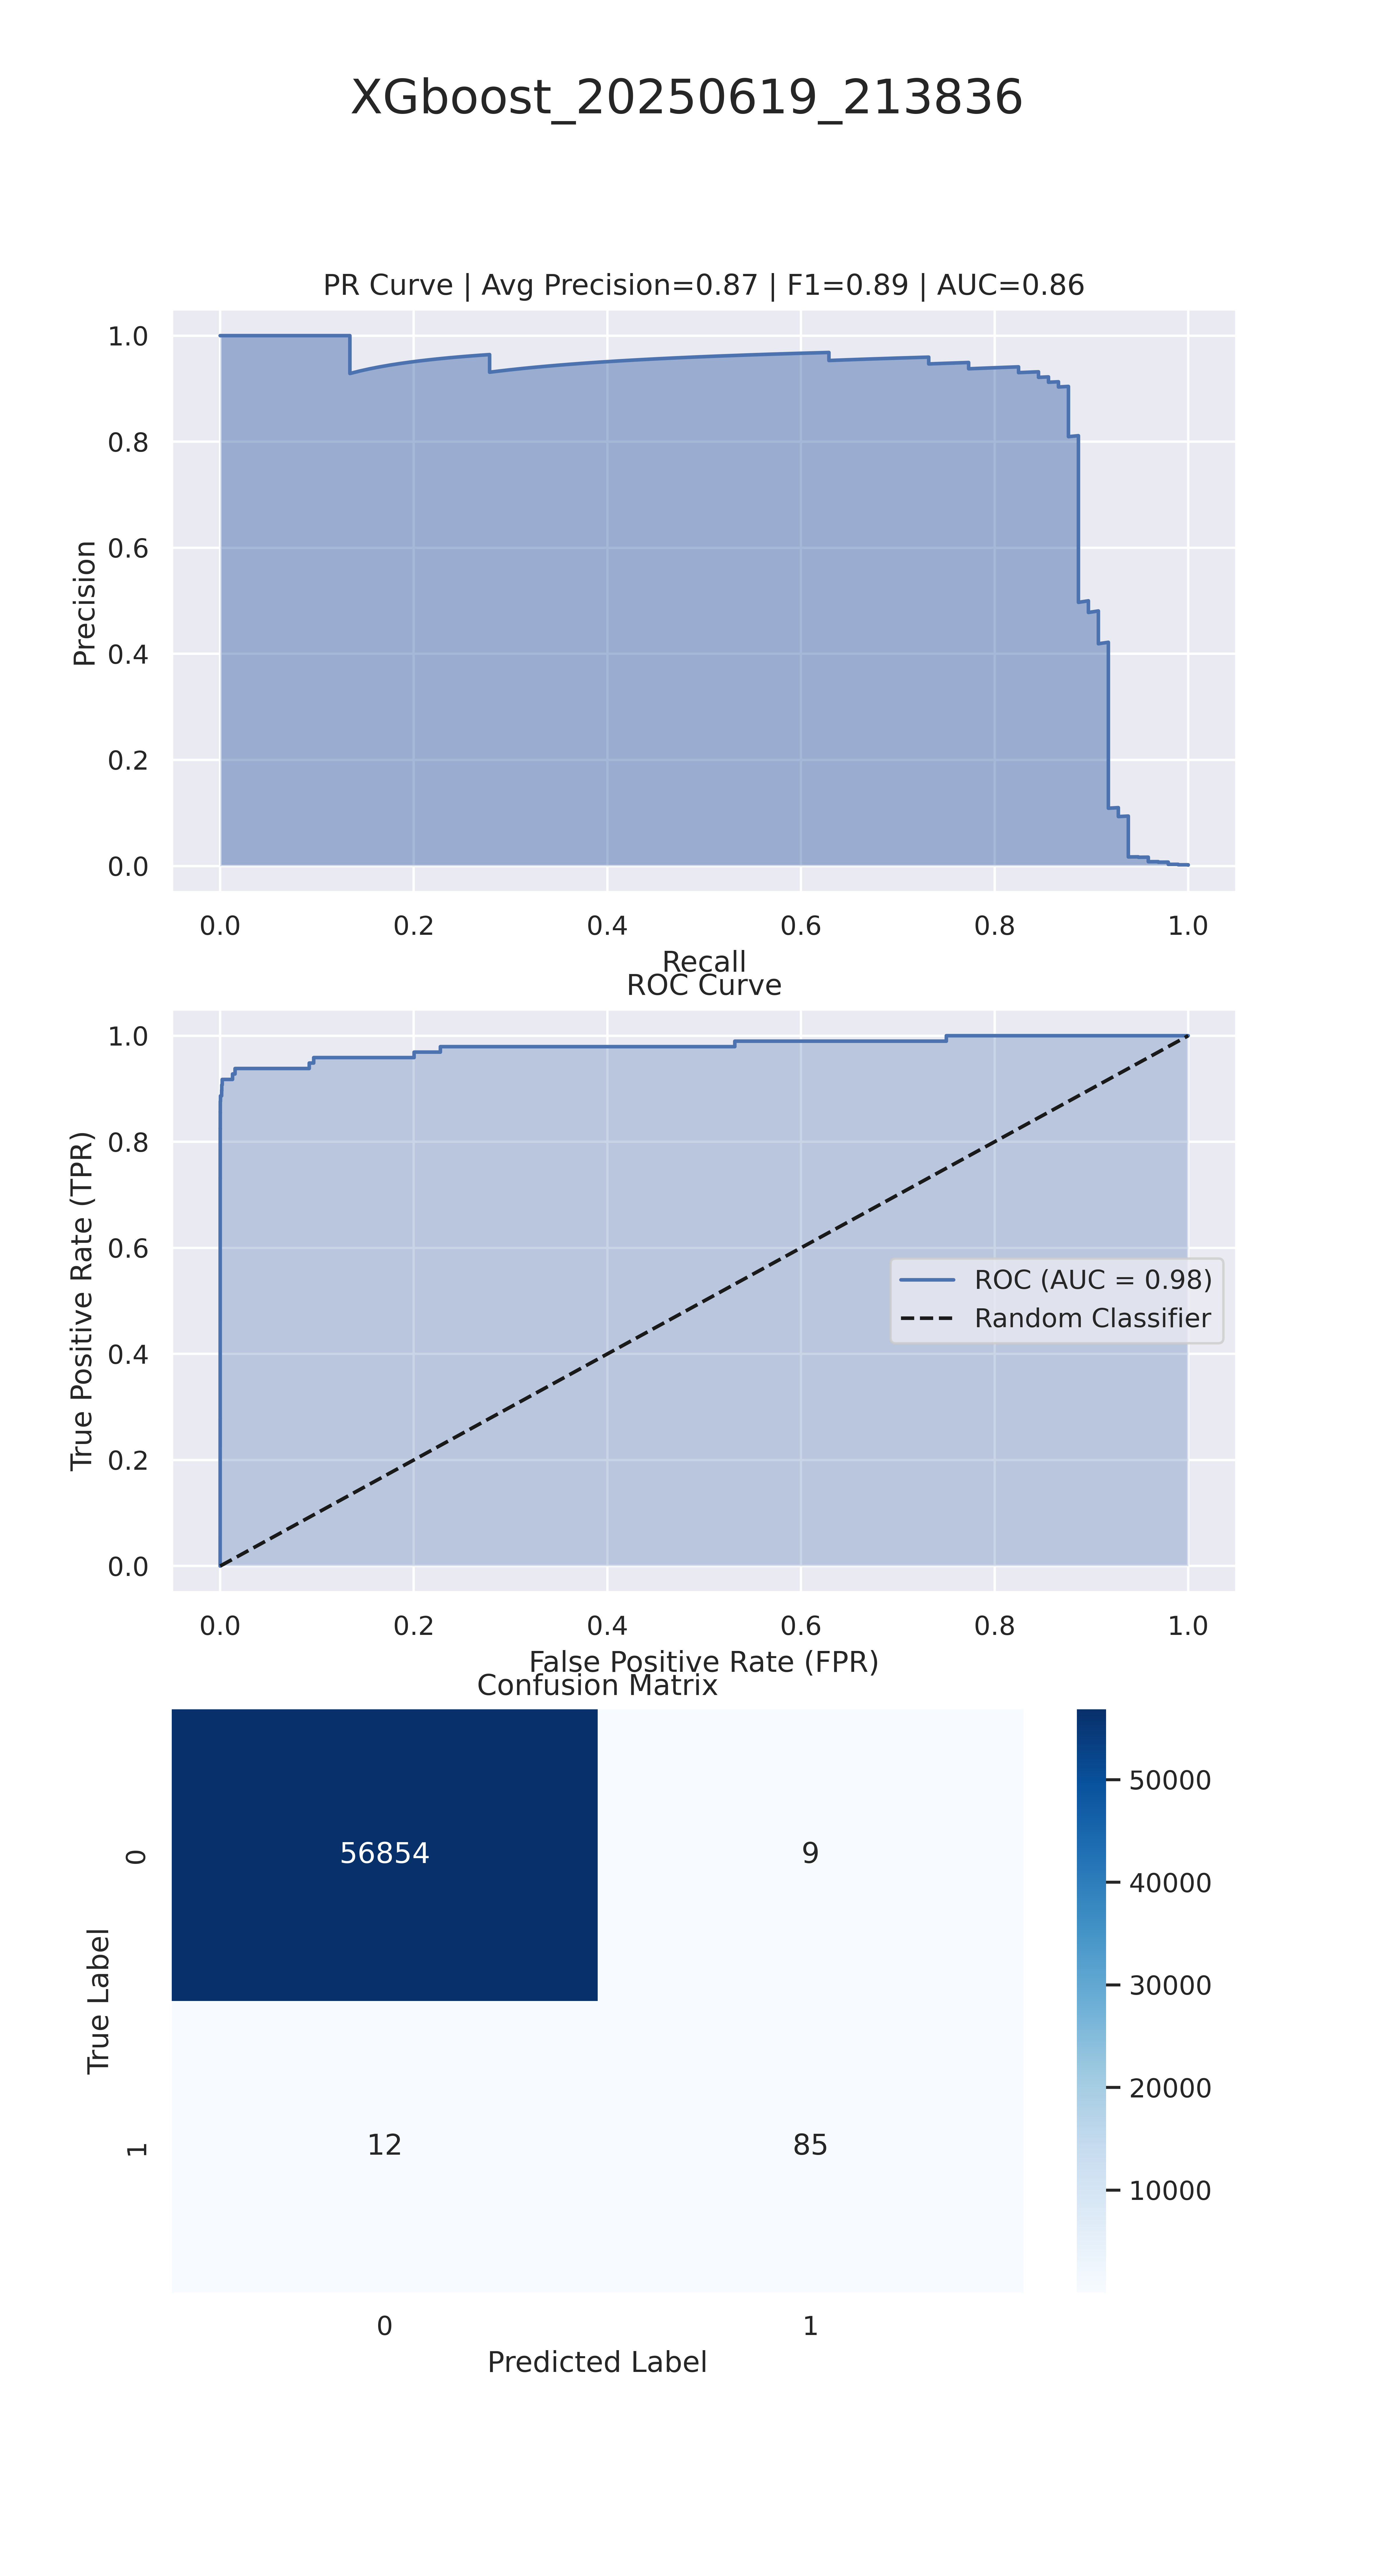
\includegraphics[width=0.95\linewidth]{XGboost_20250619_213836.png}
    \caption{Performance plots for the top-performing XGBoost model, showcasing its high AUC for both the ROC and Precision-Recall curves.}
    \label{fig:xgboost_results}
\end{figure}

A complete comparison of all evaluated models is provided in Table~\ref{tab:model_performance}, with a visual summary in the heatmap in Figure~\ref{fig:heatmap-models}.

\begin{table}[htbp]
\centering
\caption{Model performance metrics on the test set.}
\label{tab:model_performance}
\begin{tabular}{lcccc}
\toprule
\textbf{Model} & \textbf{F1} & \textbf{AP} & \textbf{ROC} & \textbf{PR} \\
\midrule
AdaBoost      & 0.85 & 0.86 & 0.98 & 0.86 \\
DecisionTree  & 0.72 & 0.70 & 0.97 & 0.79 \\
GradBoost     & 0.88 & 0.86 & 0.98 & 0.86 \\
LGBM          & 0.88 & 0.87 & 0.98 & 0.87 \\
LogReg        & 0.77 & 0.72 & 0.98 & 0.72 \\
RF            & 0.80 & 0.76 & 0.97 & 0.77 \\
XGB           & 0.89 & 0.87 & 0.98 & 0.87 \\
CatBoost      & 0.87 & 0.87 & 0.98 & 0.87 \\
LogRegFocal   & 0.75 & 0.59 & 0.92 & 0.72 \\
KNN           & 0.85 & 0.82 & 0.93 & 0.87 \\
NNFocal       & 0.77 & 0.62 & 0.92 & 0.74 \\
\bottomrule
\end{tabular}
\end{table}

\begin{figure}[htbp]
    \centering
    \includegraphics[width=0.95\linewidth]{heatmap.png}
    \caption{Evaluation of all models over the test dataset.}
    \label{fig:heatmap-models}
\end{figure}

\section{Conclusion}
\begin{itemize}[noitemsep]
    \item Tree-based and boosting models perform well on this imbalanced data.
    \item Standard logistic regression and neural networks underperform.
    \item Focal loss offers a slight improvement for these models.
\end{itemize}

\section{What Could Be Enhanced}
\begin{itemize}[noitemsep]
    \item Improve feature engineering to create more discriminative features.
    \item Use over/under-sampling techniques (SMOTE, ADASYN) to balance the training data.
    \item Carefully select a subset of high-performing, diverse models for an optimized ensemble voter.
\end{itemize}

\end{document}